% !TeX spellcheck = en_US
\documentclass[french]{yLectureNote}

\title{Atomistique 2 - PS}
\subtitle{Chimie}
\author{Paulhenry Saux}
\date{\today}
\yLanguage{Français}

\professor{J.Cunny}
\usepackage{graphicx}%----pour mettre des images
\usepackage[utf8]{inputenc}%---encodage
\usepackage{geometry}%---pour modifier les tailles et mettre a4paper
%\usepackage{awesomebox}%---pour les boites d'exercices, de pbq et de croquis ---d\'esactiv\'e pour les TP de PC
\usepackage{tikz}%---pour deiffner + d\'ependance de chemfig
% \usepackage{tabularx}%---pour dimensionner automatiquement les tableaux avec variable X
\usepackage{awesomebox}%---Pour les boites info, danger et autres
\usepackage{menukeys}%---Pour deiffner les touches de Calculatrice
\usepackage{fancyhdr}%---pour les en-t\^ete personnalis\'ees
\usepackage{blindtext}%---pour les liens
\usepackage{hyperref}%---pour les liens (\`a mettre en dernier)
\usepackage{caption}%---pour la francisation de la l\'egende table vers Tableau
\usepackage{pifont}
\usepackage{array}%---pour les tableaux
\usepackage{lipsum}
\usepackage{yFlatTable}
\usepackage{multicol}
\newcommand{\Lim}[1]{\lim\limits_{\substack{#1}}\:}
\renewcommand{\vec}{\overrightarrow}
\newcommand{\N}[0]{\mathbb{N}}
\newcommand{\dd}{\mathrm{d}}
\newcommand{\norm}[1]{||\vec{#1}||}
\newcommand{\fo}{\psi(\vec{r},t)}
\newcommand{\foe}{\psi(\vec{r},t)\*}
\newcommand{\HH}{\hat{H}}
\newcommand{\hb}{\hbar}
\newcommand{\lap}{\nabla^2}
\newcommand{\lapcc}{\frac{\partial^2 }{\partial x^2}+\frac{\partial^2 }{\partial y^2}+\frac{\partial^2 }{\partial z^2}}
\begin{document}
\setcounter{chapter}{1}
\chapter{Orbitales moléculaires}
% \section{Atomes polyélectroniques}
% \subsection{Résolution de l'équation : He}
% \subsubsection{Opérateur hamiltonien}
% On se place dans un repère dont l'origine est le noyau. 2 électrons ``gravitent'' autour. On veut résoudre l'équation de Schrödinger pour ce système. On écrit d'abord l'hamiltonien :
% \begin{flalign*}
% E &= T_{e_1} + T_{e_2} + V_{e_1N} + V_{e_2N} + V_{e_1e_2}\\
% \HH(e_1,e_2) &= \hat{T_{e_1}} + \hat{T_{e_2}} + \hat{V_{e_1N}} + \hat{V_{e_2N}} + \hat{V_{e_1e_2}}\\
% &= {\color{warningColor}-\frac{\hb^2}{2m_e}(\lap_{e_1}+\lap_{e_2})} - {\color{checkColor}\frac{2e^2}{4\pi\epsilon_0}(\frac{1}{\hat{r_1}}+\frac{1}{\hat{r_2}})} + {\color{tipsColor}\frac{e^2}{4\pi\epsilon_0}\frac{1}{\hat{r_{12}}}}
% \end{flalign*}
% \subsubsection{Simplification}
% Pour résoudre l'équation de Schrödinger, on aimerait séparer les variables pour obtenir \(\HH(e_1,e_2) = \hat{h}(e_1)+\hat{h}(e_2)\), mais c'est impossible en raison du {\color{tipsColor}dernier terme}. On va donc le supposer négligeable devant les deux autres termes. On peut maintenant écrire, en unité atomique :
% \[ \left\{\begin{matrix}
%  \hat{h_1}(e_1) = -\frac{1}{2}\lap(e_1)-\frac{2}{\hat{r_1}} \\
%  \hat{h_2}(e_2) = -\frac{1}{2}\lap(e_2)-\frac{2}{\hat{r_2}}
% \end{matrix}\right.\]
% On retrouve ainsi, en injectant chacun des 2 opérateurs dans l'équation de Schrodinger :
% \[ \left\{\begin{matrix}
%  \hat{h_1}{\color{questionColor}\phi(e_1)} = {\color{criticalColor}\epsilon_1} {\color{questionColor}\phi(e_1)} \\
%  \hat{h_2}{\color{questionColor}\phi(e_2)} = {\color{criticalColor}\epsilon_2}{\color{questionColor}\phi(e_2)}
% \end{matrix}\right.\] avec {\color{criticalColor}l'énergie} des OA et les {\color{questionColor}OA classiques} des hydrogénoides. On a séparé les variables, on en déduit que \[\HH(1,2)\phi(1)\phi(2) = (\epsilon_1+\epsilon_2)\phi_1(1)\phi_2(2)\]
% \subsubsection{Généralisation}
% On peut généraliser les équations simplifiées précédentes à un atome à \(N\) électrons :
% \[ \left\{\begin{matrix}
%   \HH(1,\dots, N) &= \sum_{i=1}^N -\frac{\lap_i}{×2}+\sum_{i=1}^N\frac{-Z_N}{\hat{r_{iN}}} = \sum_{i=1}^N\hat{h_i}(i)\\
%   \psi(1,2,\dots, N) &= \Pi^n_{i=1}\phi_i(i)\\
%   E_{tot} &= \sum_{i=1}^N\epsilon_i
% \end{matrix}\right.\]
% \subsubsection{Limite}
% Le calcul de l'énergie de première ionisation de l'atome d'He ne prend en compte l'électron qui reste. On trouve une valeur très éloignée de la valeur expérimentale. Avec la formule de l'énergie \(-13.6\frac{Z^2}{n^2}\), on trouve en fait l'énergie de deuxième ionisation. Il faut donc introduire la notion d'écrantage.
% \subsection{Principe d'exclusion de Pauli}
% \begin{theorem}[Principe de Pauli]
%  Une OA ne peut contenir que 2 électrons, différant uniquement par leur état de spin \(m_s\).
% \end{theorem}
% Ainsi, pour les deux électrons de l'atome d'hélium, les 3 premiers nombres quantiques sont égaux, seul le spin change \(m_s = \pm \frac12\).
% \subsection{Écrantage}
% \begin{theorem}[Écrantage]
% Capacité d'un électron à écranter (se mettre devant, bloquer) d'autres électrons. Les électrons les plus éloignés interagissent avec le noyau mais aussi avec les électrons placés entre lui et le noyau. Ils interagit avec un bain moyen, avec une charge effective, ressentie $Z_{eff} = Z-\sigma_j$, avec $\sigma_j$ l'écrantage.
% $\sigma_j = \sum \sigma_i$, avec $\sigma_j$ l'électron étudié et $\sigma_i$ les autres électrons.
% \end{theorem}
% On obtient donc, dans le modèle de Bhor : $E = -\frac{13.6\times Z_{eff}^2}{n_{eff}^2}$.
% Chaque électron d'un atome à un $Z_{eff}$. Ceux des électrons de Valence sont les plus importants.
% \warningInfo{Remarque}{
% Sur une m\^eme sous-couche, tous les $Z_{eff}$ sont les m\^eme.
%
% Des électrons d'une m\^eme sous-couche s'écrantent aussi.
%
% Cela décrit que le ressentie d'un électron.
% }
% Les \(\sigma\) sont obtenus expérimentalement par Slater. Dans son modèle, les fonctions d'onde ne dépendent que des coordonnées de l'électron. Les OA sont corrigées avec l'ajout du \(Z_{eff}\) et du \(n_{eff}\).
\section{Approximation et équations séculaires}
\subsection{Hamiltonien}
\subsubsection{Formule}
On cherche à déterminer la forme de l'Hamiltonien pour un atome polyelectronique ou une molécule. Ce dernier sera de la forme \[\HH = {\color{criticalColor}\hat{T_e} + \hat{T_N}} + {\color{warningColor}\hat{V_{eN}} + \hat{V_{ee}}+\hat{V_{NN}}}\] avec les {\color{criticalColor}énergies cinétiques} des électrons et des noyaux et les {\color{warningColor}potentiels} liées aux interactions électrons-électrons, électrons-noyaux, noyaux-noyaux. Ces derniers se calculent avec ces sommes :
Bien sur, il est impossible de résoudre l'équation qui en décole de manière analytique.
\subsection{Approximation de Born-Oppenheimer}
\subsubsection{Approximation}
\begin{theorem}[Approx 1 : Approximation de BO]
 Comme les noyaux sont 1800 fois plus lourds que les électrons, ces derniers s'adaptent de manière instantanée et adiabatique à tout mouvement des noyaux : les positions des noyaux sont traitées comme des paramètres.
\end{theorem}
Dans cette approximation, l'équation est résolue pour une géométrie fixe\marginTips{Puisque les coordonnées des noyaux sont considérées comme fixes. En outre, ils n'ont pas de vitesse et ne subissent pas de potentiel.}. L'hamiltonien est alors \[\HH = {\color{criticalColor}\hat{T_e}} + {\color{warningColor}\hat{V_{eN}} + \hat{V_{ee}}}\]


\subsection{Approximation orbitale}
\criticalInfo{Approximation}{Ce n'est pas négliger l'interaction electron-électron. On écrit la fonction d'onde totale comme un produit de fonction d'onde monoélectroniques, appelé Orbitale Moléculaire. On peut l'écrire mais ce n'est pas vrai, je n'ai pas le droit par la présence du terme de l'interaction electron-électron !}

L'interaction électron-électron rend la résolution impossible, c'est pourquoi on fait l'approximation orbitale : on écrit la fonction d'onde comme un produit de fonctions d'onde monoélectronique. On a alors \[\psi(e_1,e_2,\dots) = \Pi_{i=1}^n\phi_i(e_i)\] L'énergie totale est la somme des énergies des électrons : \[E = \sum_{i=1}^{OM}n_i \epsilon_i\] avec \(\epsilon_i\) l'énergie de l'électron décrit par l'OM \(\phi(i)\) et \(n_i\) l'occupation de l'OM.

Pour faire la séparation des variables, on écrit le potentiel que ressent l'électron comme un champ moyen généré par tous les autres électrons\marginWarning[Approximation de champ moyen]{Il y a toujours cette interaction e-e, mais on suppose simplement qu'il subit une interaction crée par un champ moyen d'électron.} : \(\hat{V_i}\). De cette façon, on peut écrire
\[\HH_{el} = \sum_{i=1}^n(-\frac{\lap_i}{2}+\sum_{A=1}^N \frac{-Z_A}{r_{iA}}+\hat{V_i}) = \sum_{i=1}^n \hat{h_i}\]

On considère que les \(V_i\) ne différent que par les variables sur lesquelles ils s'appliquent\marginTips{On suppose qu'ils sont une expression mathématique unique qui ne dépend pas de i, i.e. de l'électron considéré}.

Les fonctions d'onde monoélectroniques sont dons les fonctions propres d'un unique opérateur noté \(\hat{h}\)
\criticalInfo{Problème}{On introduit le problème de la self-intéraction où chaque intéraction intéagit avec le champ commun}
\subsection{LCAO (Linear Combinaison of Atomic Orbital)}
Il faut maintenant fournir une approximation simple de \[\hat{h}\phi_i = \epsilon_i\phi_i\]
On va les exprimer comme des combinaisons linéaires d'OA\marginTips{car on suppose que les atomes ne perdent pas complètement leur identité quand ils sont en molécule}:\[\phi_i = \sum_kc_{ik}\chi_{ik}\]
Pour résoudre le système (trouver les coefficients de la combinaison linéaire), on va résoudre des équations séculaires
\subsection{Équations séculaires}
\subsubsection{Cas de deux OA}
Pour rappel, on veut résoudre \[{\color{warningColor}\hat{h}}{\color{criticalColor}\phi}_i = {\color{tipsColor}\epsilon}_i{\color{criticalColor}\phi}_i\] et on sait que dans notre cas \({\color{criticalColor}\phi} = c_1{\color{checkColor}\chi_1}+c_2{\color{checkColor}\chi_2}\). Dans ces expressions, on trouve les {\color{criticalColor}orbitales molécualaires}, l'{\color{warningColor}hamiltonien monoélectronique}, {\color{tipsColor}l'énergie des orbitales moléculaires}, {\color{checkColor}les orbitales atomiques} et les coefficent de la CL. L'objectif est de déterminer ces derniers. On injecte l'expression de \(\phi\) dans l'équation :
\begin{flalign*}
\hat{h}(c_1\chi_1+c_2\chi_2) &= \epsilon(c_1\chi_1+c_2\chi_2)\\
c_1\langle\chi_1|\hat{h}|\chi_1\rangle+c_2\langle\chi_1|\hat{h}|\chi_2\rangle &= \epsilon c_1\langle\chi_1|\chi_1\rangle+\epsilon c_2 \langle\chi_1|\chi_2\rangle
\end{flalign*}
\begin{definition}[Intégrales d'équations séculaires]
\begin{itemize}
 \item Intégrales de recouvrement : \(S_{ij} = \langle\chi_i|\chi_j\rangle = S_{ji}\). On a \(S_{ii} = 1\).
 \item Intégrales Coulombiennes : \(h_{ii} = \langle\chi_i|\hat{h}|\chi_i\rangle\). Ils représentent l'énergie de l'OA \(\chi_i\) dans l'atome isolé
 \item Intégrales de résonnance : \(h_{ij} = \langle\chi_i|\hat{h}|\chi_j\rangle = h_{ji}\)
\end{itemize}
\end{definition}
On peut déduire \(h_{ij}\) des 2 autres intégrales avec
\begin{theorem}[Formule de Wolsberg]
 \[h_{ij} = 1.75\frac{h_{ii}+h_{jj}}{2}S_{ij}\]
\end{theorem}
Avec ces nouvelles notations, on peut réécire l'équation précédente. L'autre équation est obtenue en multipliant le conjugué de \(\chi_2\) et non \(\chi_1\) lors de la troisème étape. On obtient finalement les équations séculaires

Ce système peut se mettre sous forme matricielle :

\[\begin{pmatrix}
h_{11} & h_{12}  \\
h_{21}& h_{22} \\
\end{pmatrix}
\begin{pmatrix}
c_1 \\ c_2
\end{pmatrix} = \epsilon \begin{pmatrix}
1&S_{12} \\ S_{21}&1
\end{pmatrix} \begin{pmatrix}
c_1 \\ c_2
\end{pmatrix}\] avec la matrice hamiltonienne et la matrice de recouvrement.
Nous le résoudrons dans la prochaine partie.
\section{Système séculaire}
% SIn on prend 2 OA identiques portées par 2 atomes identiques : \(h_{11} = h_{22}, h_{12} = h_{21}, S_{12} = S_{21}\).
%
% Le déterminant du systèmes est alors \((h_{11}-\epsilon)^2 = (h_{12}-\epsilon S_{12})^2\), donc \(h_{11}-\epsilon = \pm (h_{12}-\epsilon S_{12})\)
%
% On en déduit les 2 valeurs de \(\epsilon\) :
% \[ \left\{\begin{matrix}
%  \epsilon^- &= \frac{h_{11}+h_{12}}{1+S_{12}}\\
%   \epsilon^+ &= \frac{h_{11}-h_{12}}{1-S}\\
% \end{matrix}\right.\]
\subsection{Résolution}
Si on on prend 2 OA identiques portées par 2 atomes identiques : \(h_{11} = h_{22}, h_{12} = h_{21}, S_{12} = S_{21}\).

\subsubsection{Valeurs propres}
\begin{theorem}[Combinaison de n OA]
 La combinaison linéaire de n OA conduit à n OM.
\end{theorem}
Le système s'écrit alors
\[\begin{pmatrix}
h_{11}-\epsilon & h_{12}-\epsilon S  \\
h_{12}-\epsilon S & h_{11}-\epsilon \\
\end{pmatrix}
\begin{pmatrix}
c_1 \\ c_2
\end{pmatrix} = \begin{pmatrix}
0 \\ 0
\end{pmatrix}\] Pour que le système admette des solutions, son déterminant doit \^etre nul. C'est le cas si \(h_{11}-\epsilon = h_{12}-\epsilon S\) ou \(h_{11}-\epsilon = -h_{12}+\epsilon S\). On obtient
\begin{flalign*}
h_{11}-h_{12} &= -\epsilon S + \epsilon\\
\epsilon(1-S) &= h_{11}-h_{12}\\
\epsilon &= \frac{h_{11}-h_{12}}{1-S}\\
\epsilon &= \frac{h_{11}-h_{12}+h_{11}S-h_{11}S}{1-S}\\
\epsilon &= h_{11}+\frac{-h_{12}+h_{11}S}{1-S}\\
\end{flalign*}
Les 2 expressions de \(\epsilon\) sont
\[ \left\{\begin{matrix}
 \epsilon^- &= h_{11}+\frac{h_{11}S-h_{12}}{1-S}\\
  \epsilon^+ &= h_{11}-\frac{h_{11}S-h_{12}}{1+S}\\
\end{matrix}\right.\]
\subsubsection{Fonctions propres}
Résolvons le système pour trouver les constantes puis les fonctions d'ondes. Commençons avec \(\epsilon^+\)\marginInfo{On a pris la première équation sécualire mais le résultat doit \^etre le m\^eme avec la seconde} :
\begin{flalign*}
c_1h_{11}+c_2h_{12} = (h_{11}-\frac{h_{11}S-h_{12}}{1+S})c_1 &+ (h_{11}-\frac{h_{11}S-h_{12}}{1+S})c_2S\\
c_2h_{12} &= -\frac{h_{11}-h_{12}}{1+S}c_1 + h_{11}c_2S-\frac{h_{11}S-h_{12}}{1+S}c_2S\\
c_2h_{12}-h_{11}c_2S &= -\frac{h_{11}S-h_{12}}{1+S}c_1-\frac{h_{11}-h_{12}}{1+S}c_2S\\
(1+S)(c_2h_{12}-h_{11}c_2S) &= -(h_{11}S-h_{12})c_1-(h_{11}S-h_{12}-h_{12})c_2S\\
c_{2}h_{12}-h_{11}c_2S+c_2h_{12}S-h_{11}c_2S^2 &= -c_1h_{11}S+c_1h_{12}-c_2h_{11}S^2+c_2Sh{12}\\
c_2h_{12}-h_{11}c_2S &= -c_1h_{11}S+c_1h_{12}\\
c_2(h_12-h_{11}S)&=c_1(h_{12}-h_{11}S)\\
c_1&=c_2
\end{flalign*}
On en déduit que \[\phi^+ = c_1(\chi_1+\chi_2)\]
On utilise la condition de normailsation pour déterminer l'expression de \(c_1\) :
\begin{flalign*}
\langle\phi^+|\phi^+\rangle &= 1\\
c_1^2\langle\chi_1+\chi_2|\chi_1+\chi_2\rangle &= 1\\
c_1^2(\langle\chi_1|\chi_1\rangle+2\langle\chi_1|\chi_2\rangle+\langle\chi_2|\chi_2\rangle) &= 1\\
c_1^2(2+2S) &= 1\\
c_1 &=\pm \frac{1}{\sqrt{2(1+S)}}
\end{flalign*}
L'expression finale est donc \[\phi^+ = \pm \frac{1}{\sqrt{2(1+S)}}(\chi_1+\chi_2)\]
De la m\^eme façon, on trouve que\marginTips{En effet, \(c_1=-c_2\)} \[\phi^- = \pm \frac{1}{\sqrt{2(1-S)}}(\chi_1-\chi_2)\]
\warningInfo{Méthode}{On fait en fait une diagonalisation de la matrice hamiltonienne.}
\subsection{Représentation schématique}
\subsubsection{Approximation}
En apprximant la formule de Wolsberg\marginCritical{Ici, \(h_{11} = h_{22}\) car on suppose que les OA sont du m\^eme type}, on a
\begin{flalign*}
\epsilon^- &\simeq h_{11} + \frac{h_{11}S-1.75\frac{h_{11}+h_{11}}{2}S}{1-S}\\
&\simeq h_{11}+\frac{h_{11}S-1.75h_{11}S}{1-S}\\
&\simeq h_{11}+\frac{h_{11}S(1-1.75)}{1-S}\\
& = h_{11}+\Delta\epsilon^-
\end{flalign*}
De la m\^ema façon \[\epsilon^+ \simeq -\frac{h_{11}S(1-1.75)}{1+S} = h_{11}-\Delta\epsilon^+\]
\subsection{Propriétés}
\begin{theorem}[Ordre de Liaison]
$p = \frac{N_{eL}-N_{eAL}}{2}$. Si p=0, la molécule est instable.
\end{theorem}
\begin{theorem}[Stabilisation dans le cas disymétrique]
 \[\Delta \epsilon^+ \propto \frac{S^2}{h_{11}-h_{22}}\]
\end{theorem}
\subsection{Diagrammes à connaitre}
Diagramme HeH :

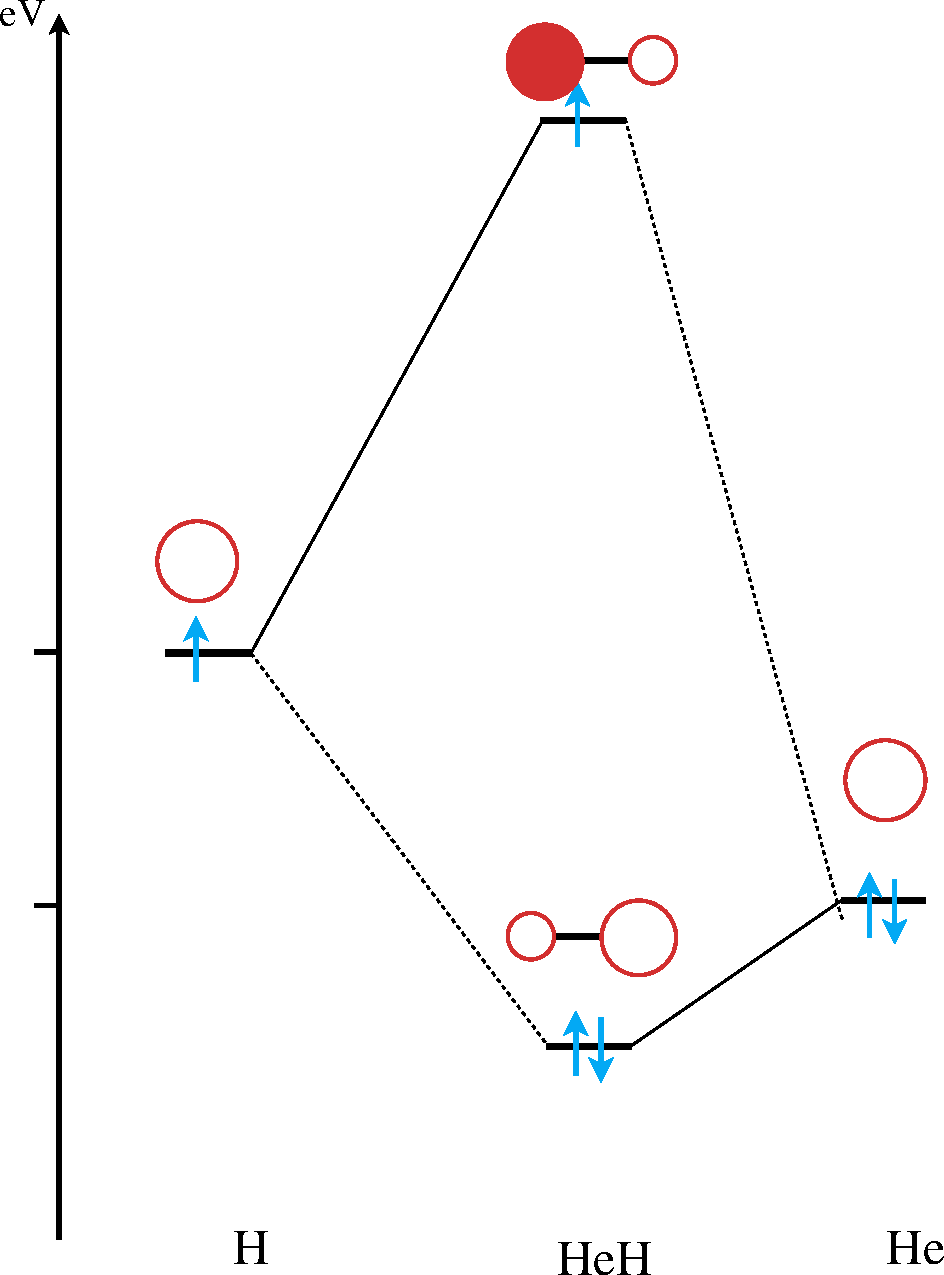
\includegraphics[scale=0.5]{DOM_HeH}

Diagramme LiH :

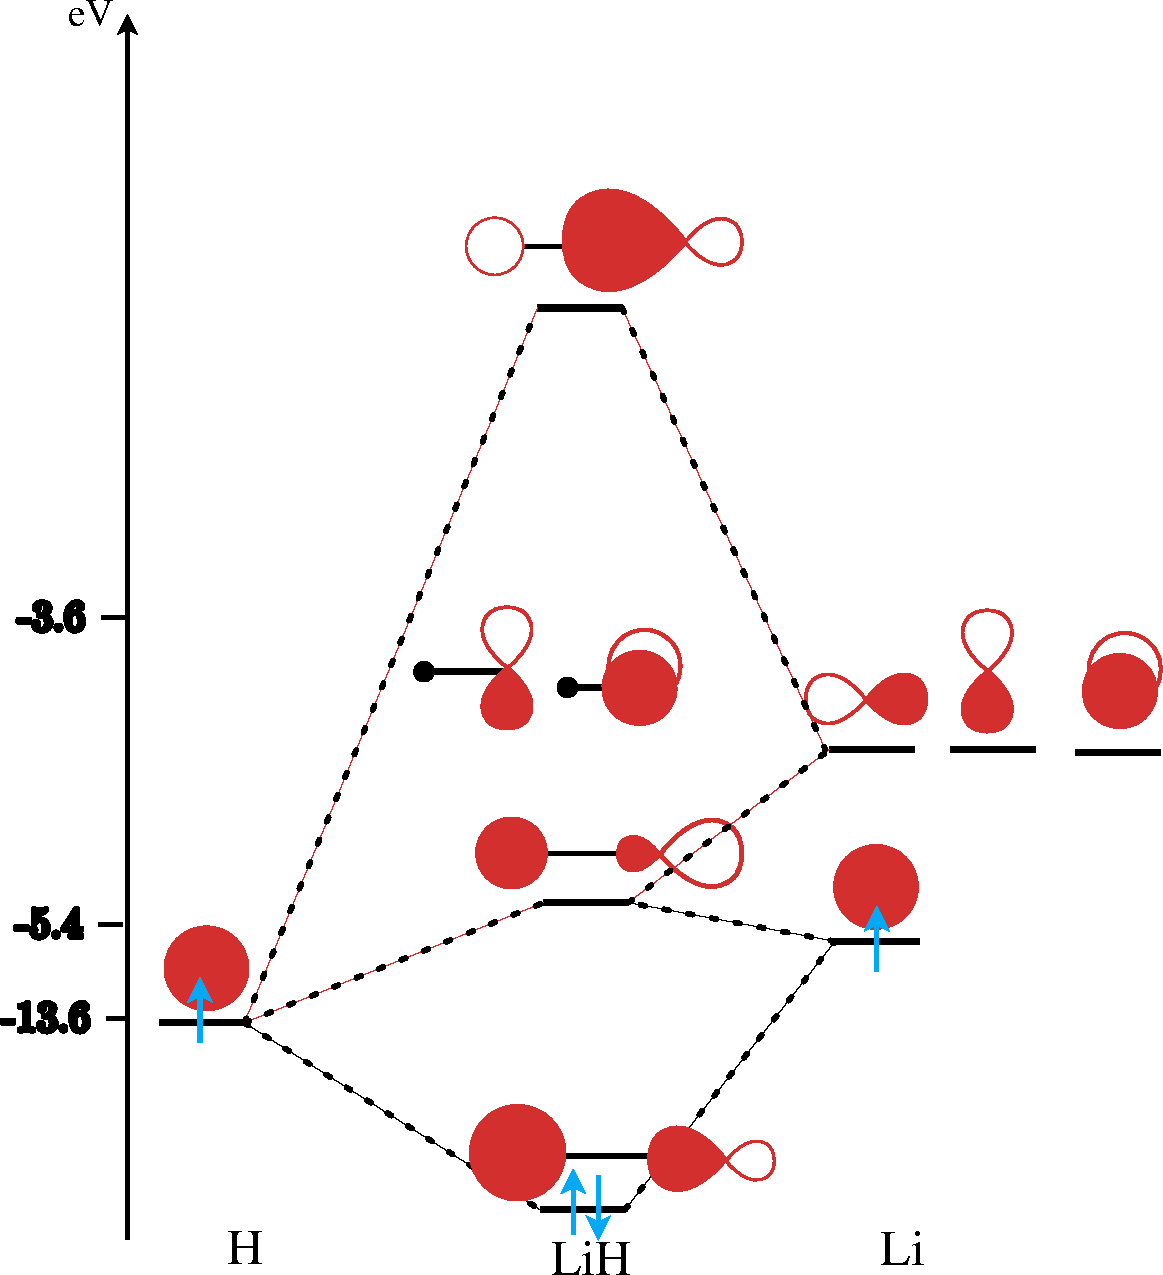
\includegraphics[scale=0.5]{DOM_LIh}
\section{Diagramme d'orbitales moléculaires}
%\subsection{Formulation matricielle}

\subsection{Recouvrements}
\begin{proposition}[Recouvrement]
Si S = 0, deux OA ne forment pas d'OM. Si 2 OA sont portées par le m\^eme atome, elles ne forment pas d'OM. En somme, 2 OA avec des symétries différentes auront un recouvrement nul
\end{proposition}
La valeur de S dépend de la nature des OA, de leur orientation et de la distance entre atomes portants ces OA.
\begin{center}
\begin{tabular}{lll}
OA & Type de recouvrement & Type d'OM\\
s/s & axial & \(\sigma\)\\
s/p axial & axial & \(\sigma\)\\
s/p latéral & \(\varnothing\) & \(\varnothing\)\\
p/p axial & axial & \(\sigma\)\\
p/p axial/latéral & \(\varnothing\) & \(\varnothing\)\\
p/p latéral & latéral & \(\pi\)\\
s/d axial & axial & \(\sigma\)\\
s/d 45° & \(\varnothing\) & \(\varnothing\)
\end{tabular}
\end{center}
L'élatement \(\pi\) est plus faible que l'éclatement \(\sigma\)
\subsection{Orbitales}
Les OA à considérer dans la LCAO sont :
\begin{proposition}[OA à considérer]
\begin{itemize}
 \item H/He : 1s
 \item bloc s et p : ns + np
 %\item bloc p : ns + np
% \item bloc d : ns + np + (n-1)d Pas besoin ce semestre
\end{itemize}
n représente le niveau de l'électron  le plus haut.
\end{proposition}
\begin{theorem}[Règle de 15 eV]
 Les OA séparées de plus de 15 eV environ ne forment pas d'OM. En conséquences, il n'y a pas d'interaction entre OA de valence et OA de coeur.
\end{theorem}
% \subsection{Systèmes Pi}
% Il faut différencier le système \(\pi\) et \(\sigma\) de la molécule\marginInfo{En effet, ces 2 systèmes sont traités indépendamment lors de la consruction du DOM}.
% On distingue ainsi 2 types de liaison :
% \begin{itemize}
%  \item Liaison $\sigma$ : Intéraction entre 2 OA avec une symétrie de révolution le long de l'axe de la liaison\marginInfo{L'OA ne change pas tout autour de l'axe}.
%  \item Liaison $\pi$ : Intéraction entre 2 OA présentant un plan d'antisymétrie contenant l'axe de la liaison\marginInfo{Il s'agit d'un plan de symétrie mais avec un changement de signe des OA par la symétrie}. Elles sont d'une énergie plus faible que les liaisons $\sigma$ mais peuvent se délocaliser.\marginCritical{Ce sont les seules à pouvoir le faire. Les liaisons $\sigma$ ne le font pas ou extrêmement rarement.}
% \end{itemize}
\subsection{Interaction à 3 orbitales}
On crée 3 OM\marginTips{EN effet, comme on l'a vu plus haut, n OA donnent n OM}. La première est totalement liante, la dernière est anti-liante. Enfin, celle du milieu est globalement non-liante\marginInfo{En effet, elle est le fruit d'une interaction antiliante et d'une liante.}

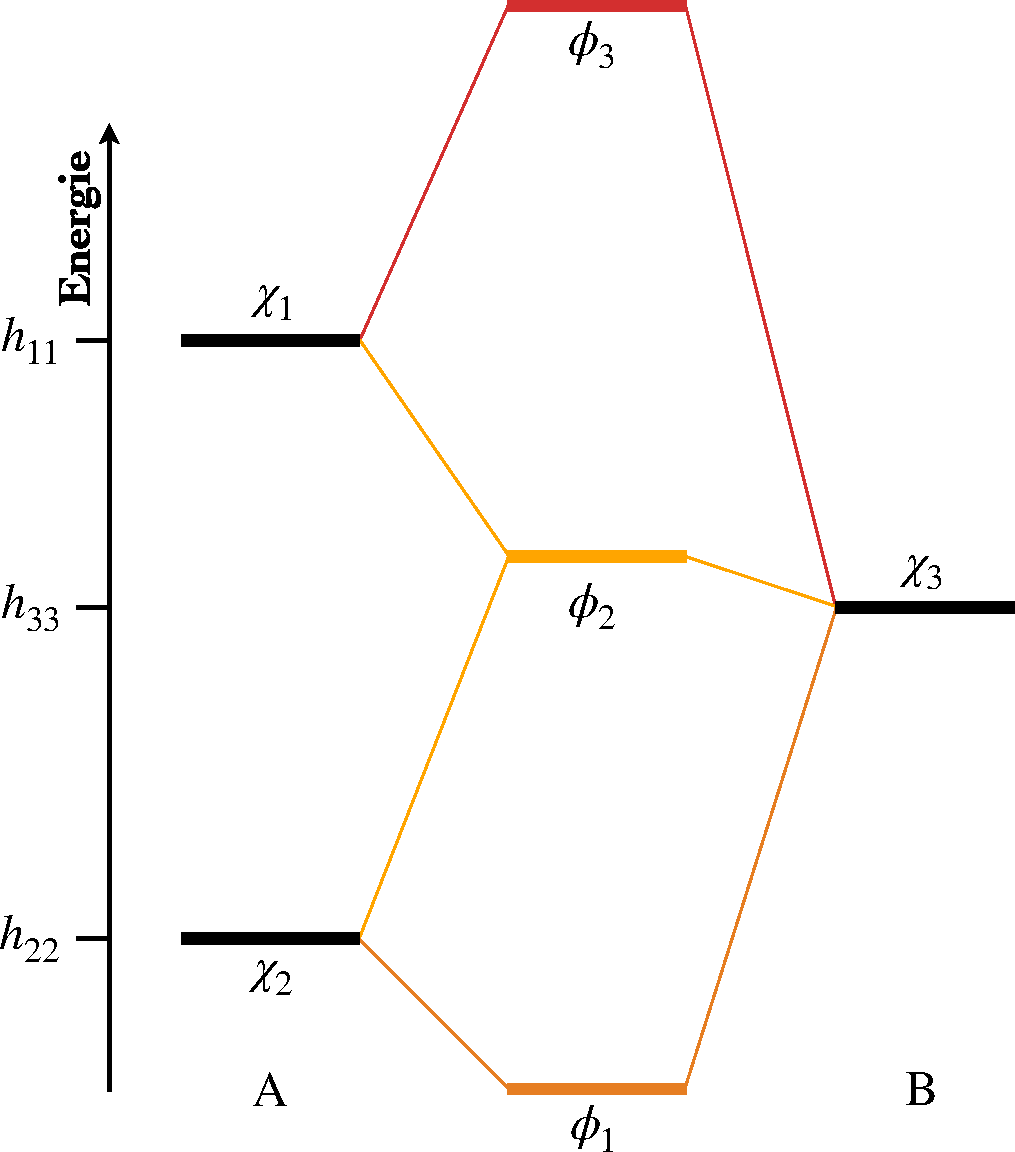
\includegraphics[scale=0.25]{figures/DOM_3}

\criticalInfo{Intéraction du milieu}{Pour une intéraction à 3, l'OM du milieu est produite par l'intéraction du bas anti-liante et celle du haut est liante.}
\subsection{Méthode des fragments}
\subsubsection{Principe}
Pour une molécule avec 3 centres ou plus, on découpe en deux fragements fictifs\marginInfo{Ces fragment n'ont pas à avoir une réalité physique ou chimique. C'est simplement un découpage.}
Il faut respecter au maximum la symétrie de la molécule\marginInfo{Toutes les fragmentations sont justes, il faut juste choisir celle qui conduit au DOM le plus simple}.
\subsubsection{Exemple avec BeH2 et H2O}
On peut séparer en HBe + H ou en HH + Be. Comme on veut conserver la symétrie de la molécule, on prend la seconde séparation. On va donc faire le DOM avec les OA de Be et les OM de $H_2$. On obtient\marginTips{On indique avec la lettre u ou g en indice si l'OM possède un centre de symétrie ou un centre d'anti-symétrie. On note AL les OM anti-liantes, NL les OM non-liantes, et L les OM liantes} :

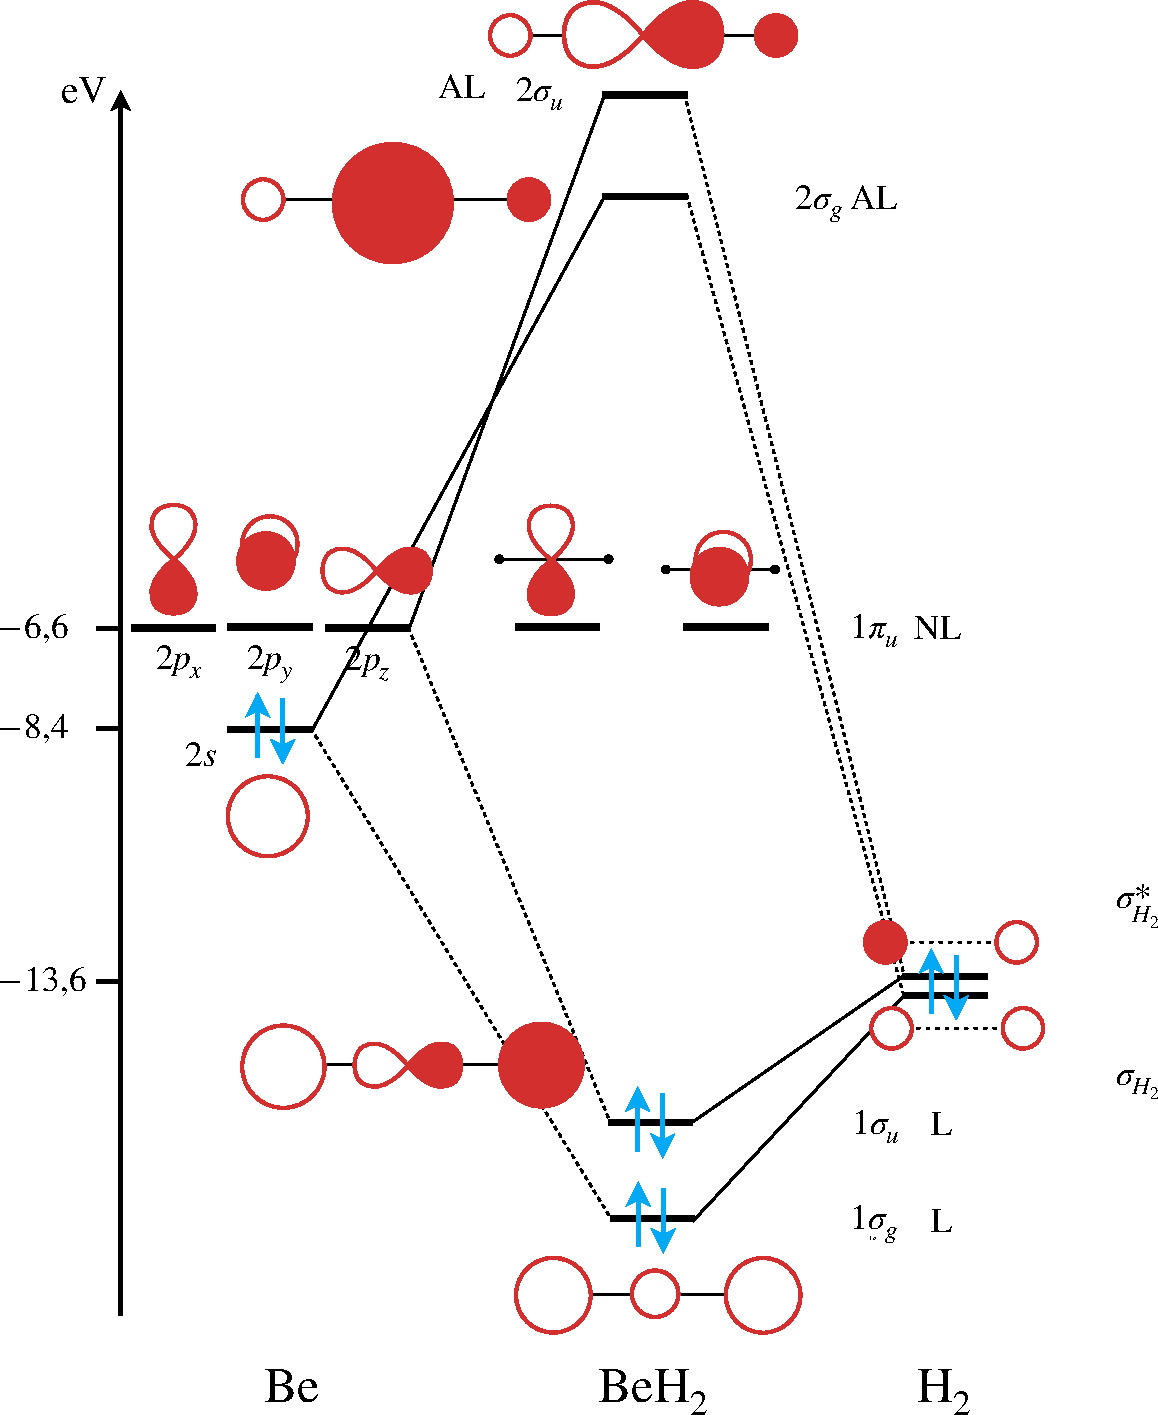
\includegraphics[scale=0.5]{figures/DOM_BeH2}

On fait de la m\^eme façon pour H2O\marginCritical{Ici, on n'a pas appliqué la règle des 15 eV afin d'obtenir un DOM exact.} :

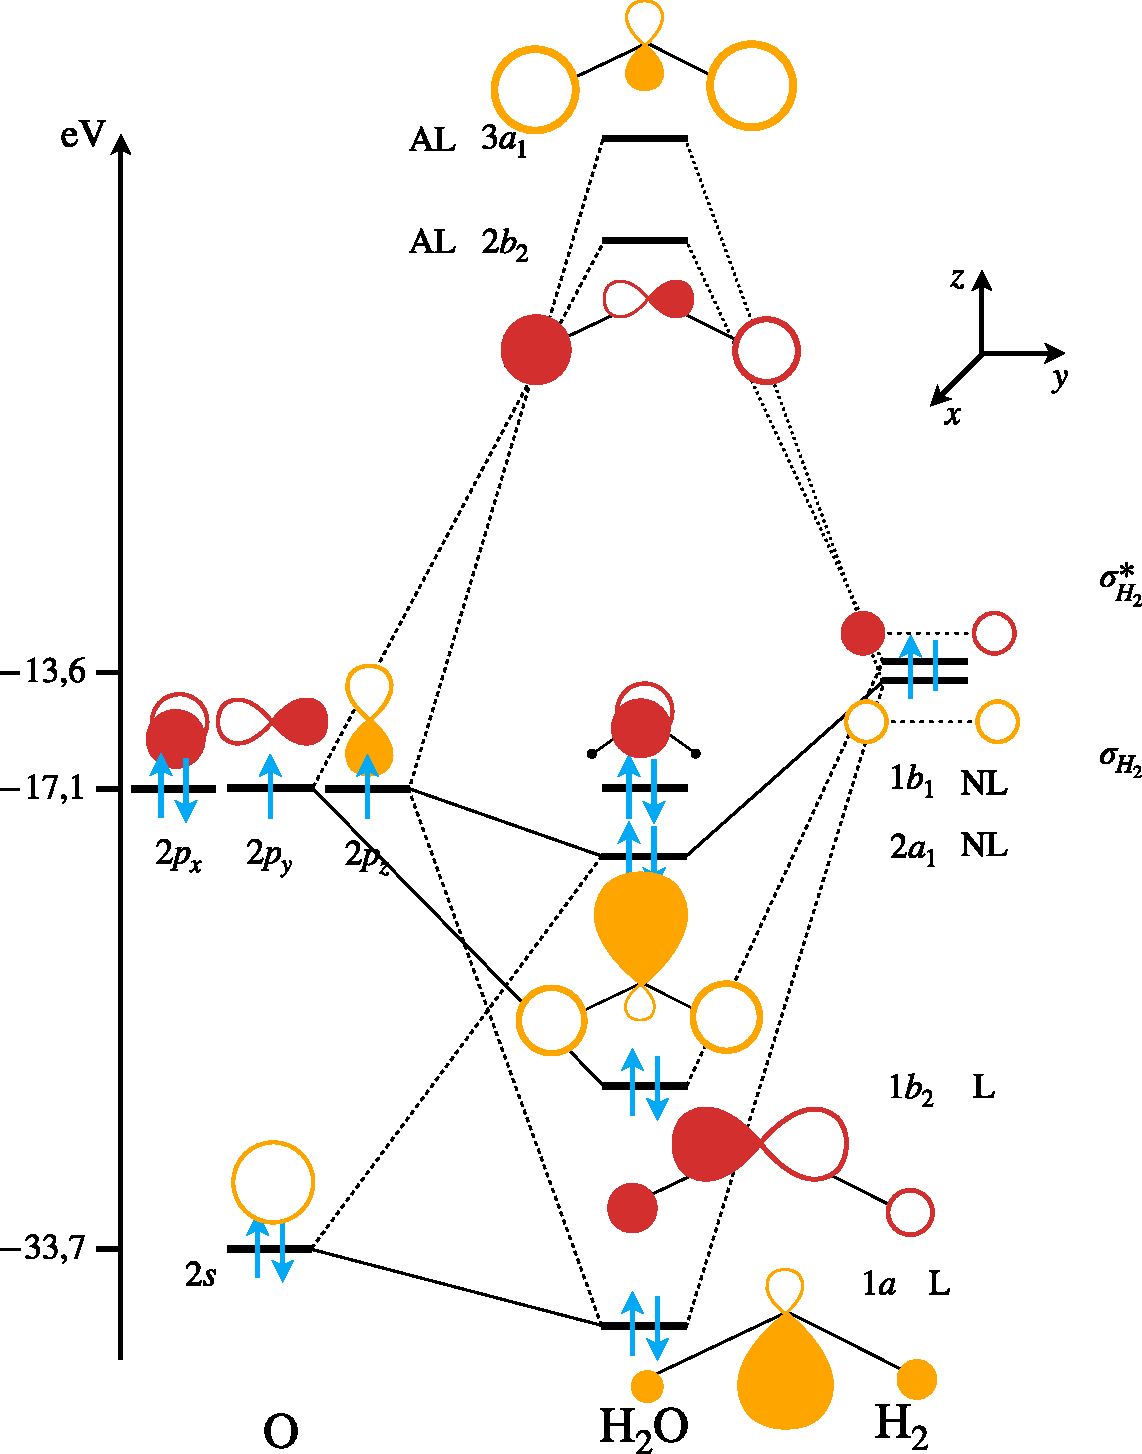
\includegraphics[scale=0.5]{figures/DOM_H2O}
 \end{document}
